\documentclass{article}
\usepackage[utf8]{inputenc}
\usepackage{hyperref}
\usepackage{nameref}
\usepackage{graphicx}
\usepackage{caption}


%\newcommand*{\fullref}[1]{\hyperref[{#1}]{\autoref*{#1} \nameref*{#1}}}
\setlength{\parindent}{0pt}
\usepackage[left=3cm,right=3cm,top=1.5cm,bottom=1cm]{geometry}



\title{Once apone a time}
\author{Rikard Helgegren}
\date{November 2015}

\begin{document}

\maketitle
\tableofcontents 
\newpage
\section{How to make a book}

\subsection{Tips}
\begin{description}
\item[Name generators for inspiration]
\item[Do your research so you know what you write about]
\item[Don't make a perfect world, it needs to be fixed]
\item[Don't make a perfect character, some flaws involved] Make a background story for every character whit a name.
\item[force the character out of their comfortzone \{makes them strugle and grow\} ]
\item[write down what you would do in a situation and compare it.]
\item[Start shaping things from the ground and add detail to them bit after bit.]
\end{description}
\subsection{why do i write this book, \{makes me find motivation\}}
I really want to be the creator of a world.
I like to try new stuff. .ui


\subsection{Is the book in the past, the present or in the future?} "The past" or we don't need to connect it whit this world, but it should be medieval.

\subsection{How did the world come to exist/ What past event have shaped it? i.e a timeline} The \nameref{troll}s have for centuries lived in Harmony with/in the \nameref{forest1}. But the \nameref{cyclops} have begun to raid and make chaos in this world.

\subsection{How does your story ends. make a timeline}


\subsection{Answers to questions}
\label{question}
\begin{description}
\item[Rules and punishment]
\item[Government/Ruler]
\item[What does the society value]
\item[\ ]
\item[Daily work/school]
\item[Food/eat]
\item[how do they play/enjoy themselves]
\item[how treat yung and old]
\item[relation to animals and plant]
\item[How do the plants and animals look]
\item[technology]
\item[transportation]
\item[communication]
\item[trades whit others]
\item[attitude towards other towns]
\item[Access to information/books]
\item[Wealth of the region]
\item[how does magic work] Gained by saving an other beings life?
\end{description}

\subsection{Create a pool of characters}

\subsection{--Name--} 
\textbf{Role:} ex. The protagonist
\\\textbf{speeches:} 
\\\textbf{sex, age, height, body type, face}
\\\textbf{Motivation:}
\\\textbf{Life experience:} 
\\\textbf{Strengths:}  
\\\textbf{Weaknesses:} 
\\\textbf{Background story:}
\\\textbf{Relationship to family and what the family is like:}
\\\textbf{friends types:}
\\\textbf{Skills:}
\\\textbf{Fears and securities:} 


\subsection{Make a map over the town/the area}

\subsection{Set a character free in the world an see what happens in a normal day}

\begin{description}
\item[how does the world shape the characters in it] 
\end{description}


%------------- Keep my fact straight
\newpage
\section{Plot line}
\subsection{Village raid}
The pygmy tribe have been out and gathered food, everyone except \nameref{Viska} have returned when a band of \nameref{cyclops} attacks the village to turn the villagers to slaves.

\subsection{Leav the forest}\nameref{Viska} knows a lot about the \nameref{cyclops} and understands that she can't save them all by her self. (Since she's not outgoing she this will be a problem)

\subsection{Problem} \nameref{Viska} have problems surviving outside the forest because she don't know what is eatable and how to prepare the food. sees 

\section{The World}
\label{world}
It is much vegetation which as consequence results in much higher oxygen levels. Which makes fires more intensive and it the "condition" of animals over all is better.


\begin{figure}[h!]
\centering
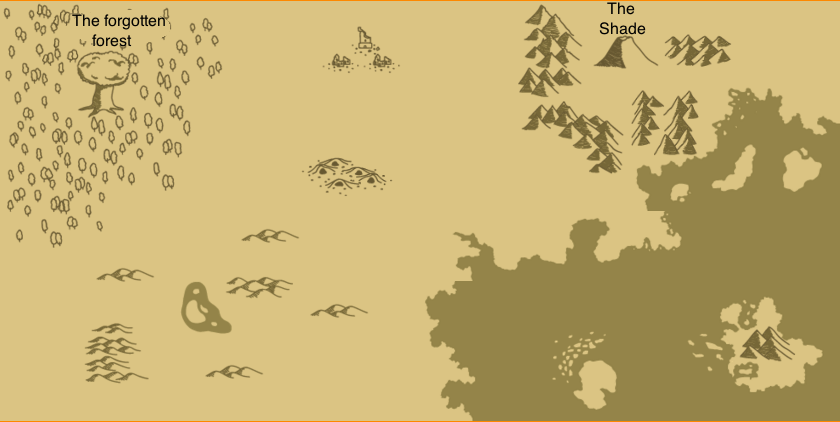
\includegraphics[width=150mm]{world.png}
\caption*{A map over the world with \nameref{forest1} in the top left corner and \nameref{volcano1} in the top right corner.}
\end{figure}
\begin{figure}[h!]
\centering
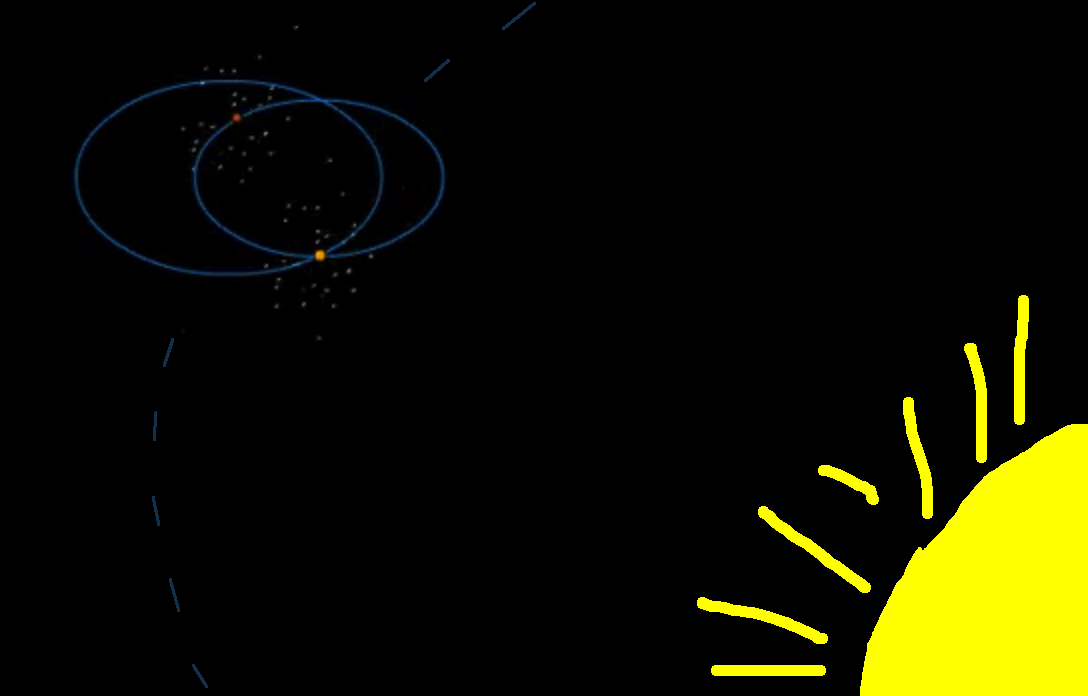
\includegraphics[width=150mm]{World+.png}
\caption*{An disproportional sketch over the solarsystem}
\end{figure}

\section{Locations}%%%%%%%%%%%%%%%%%%%%%%%%%%%%%%%%%%%%%%%%%%%%%%%%%%%%%%%%%%%%%%%%%%%


% A place where all optical illusions are for real. ""










\subsection{The forgotten forest}
\label{forest1}

\textbf{Description:} \nameref{forest1} is a old forest with many huge trees. The wind is whispering in the leafs for the inhabitants to hear. Most of the trees in \nameref{forest1} are deciduous and have vines dangling from the foliage. The ground is covered in a thick layer of grassgreen moss, and bunches of mushrooms in various colours are spread. In the middle of the forest is the \nameref{big tree}\\
\textbf{Weather:} This is played out in the summer when it's 35 $^\circ C$ at noon and 30 $^\circ C$ during the night. Due to all the trees that keeps the warmth. It rains a bit every morning, and the humidity is high.


\textbf{Animals:} Moose, bear, rabbits

\textbf{Extra fact:} In the skirts of \nameref{forest1} their lives a tribe of \nameref{troll}s.
%---------------------------------------------------
\subsection{The shade}
\label{volcano1}
\textbf{Description:} \nameref{volcano1} is a sky high active volcano with lavapools at its feet. The sky is hidden behind a thick sheet of smoke and the nose stings due to the smell of sulfur. The covering layer of soot makes that that there is only one living plant in this area, the \nameref{dust bush}.
%The boiling of lava is easily heard  
\\\textbf{Weather:} It rarly rains since the mountains around are so high.
\\\textbf{Animals:} \nameref{worms}, \nameref{lizard}, \nameref{cyclops} 

\textbf{Extra fact:} In large tunnel system the \nameref{cyclops} have their site.
%---------------------------------------------------

\section{Animals}%%%%%%%%%%%%%%%%%%%%%%%%%%%%%%%%%%%%%%%%%%%%%%%%%%%%%%%%%%%%%%%%%%%
\subsection{Pygmy-Troll}
\label{troll}
\textbf{Description:} The troll is a short, almost figure eighth being. The compact rubberlike torso in combination with their long tail make them excellent at bouncing as they please. they have short legs and unproportionally large feet. Their round nose, big eyes and big chins makes them lock very friendly, which they are. They have also a high intelect and thusly there is no need for rules in the tribe\\ 
\textbf{Location:} These trolls live in \nameref{forest1}.\\
\textbf{Height:} 140 cm as fully grown.\\
\textbf{Diet:} Herbivores. They eat fruits, leafs and shoots from trees and bushes, mushrooms 
\\\textbf{Movement: } The fastest way for a \nameref{troll} to move is to bounce in a waddleling-way back an forth. They use their big feet to gain both speed and height in their movement and steer whit the tail. They can also walk if they want to sneak, but it's a slow process since they have no legs.
\\\textbf{Sleep:} They only sleep 3 to 4 hours every night.
\\\textbf{Communication: } Via talk or if they lean their head angainst eatch other to enable the other troll to read their thoughts.
\\\textbf{Attitude towards other speeces} Non-hostile
\textbf{Tribe leader:}
The tribe leader is the oldest willingly woman. When a tribe leader decides to make unity with the earth (die). A new woman will take her place




\iffalse
\textbf{Rules:}
\begin{enumerate}
  \item It's forbidden to hurt someone on purpose.
  \item It's forbidden to steal from someone.
  \item It's forbidden to make a bonfire without having a stone ring around it.
\end{enumerate}
\fi



\textbf{Daily work}
Everyone gathers what food will be needed for that day, except for the youngest and the oldest. The oldest babysits youngest during this time and booth learn from and teach the young. When a young troll is old enough i.e learned to bounce properly and communicate without head contact, then their parents take them along to show them the forest where to gather fruits and other vegetables.
When the gathering is done it's up to each individual what they want to do. Many trolls at this time improve different skills or do what they enjoy (climbing and dropping from trees, interact whit other animals, experiment with food, write songs or tales, juggle, swim in the lake, practise a instrument, a trip in the forest \{maybe to the \nameref{big tree}\}).
In the evening the tribe gather around a bonfire, sings, dances, tell stories and talk before they go to sleep.

\textbf{Dying: } When a troll decides it's time to leave this world the tribe walks to the \nameref{big tree}. They connect their heads too share the last goodbye of the troll. After the goodbye a wind is whispering trough the leafs, the troll fades a way and its spirit follows the wind.




%--------------------------------------------------
\subsection{Cyclops}
\label{cyclops}

\textbf{Description:} The cyclops could be mistaken for a tall muscular human at a large distance if it wasn't for their pointy bonewhite horns. At a close range one can easily see the veins pulsing on the defined muscles. With the long sharp teeth, claw like nails and thick skin, the cyclops is the most dangerous predator in \nameref{world}. The stained blood on the skin makes the cyclops smell rotten. Cyclops livs and hunts in packs up to 12 but more comon is groups of 5 due to that a cyclop is easily iritated and have a hot temper.    
\\\textbf{Location:} The cyclops have their origin at \nameref{volcano1}, but cyclops have been plundering and kidnapping for many years in other parts of \nameref{world}
\\\textbf{Height:} 210 cm as fully grown.
\\\textbf{Diet:} flesh and carcass. (\nameref{lizard} when at \nameref{volcano1})
\\\textbf{Movement: } They move as humans.
\\\textbf{Sleep: } same sleep patterns as humans
\\\textbf{Attitude towards other speeces} Hostile
\\\textbf{The alfa leader:} Is the one best at cyclop vs cyclop
\\\textbf{dying} A cyclop gets often killed by other groups of cyclops if they look weak or crippled. The only exception is infants who is protected by younger mebers in a group/pack
%--------------------------------------------------
\subsection{Fagris}
\label{lizard}

\textbf{Description: } Their hard scales are black whit red edges. They have a triangular head with rows of spikes that starts on the forehead and  goes along to the tail. Their slim figure and sharp claws make them good at climbing in the mountains, or dig for \nameref{worms}. The \nameref{lizard} green eyes are only good at detecting motions during the night and too sensitive during the day.
\\\textbf{Location: }\nameref{volcano1}
\\\textbf{Diet: }\nameref{worms}s or other animals
\\\textbf{Length: } 160 cm from tail to nose.
\\\textbf{Movement: } walks/runs on all for.
\\\textbf{Sleep: } Sleeps in holes during the day.

%--------------------------------------------------
\subsection{Magma worm}
\label{worms}

\textbf{Description: } A \nameref{worms} is like a large maggot, the difference is mainly that the \nameref{worms} have several teeth in their cylindrical mouth, sharp and strong enough to crush magma stones and dig tunnels 
\\\textbf{Location: }\nameref{volcano1}
\\\textbf{Diet: }\nameref{dust bush}es and magma stones
\\\textbf{Circumference: } 30 cm and length 1 m.
\\\textbf{Movement: } They have small legs at the front but they manly move by contracting and expanding its body. It have a top speed at 5 km/h
\\\textbf{Sleep: } Is most active between dusk and dawn but can dig tunnels any time.

\iffalse
%--------------------------------------------------

\subsection{Gladier}

\textbf{Description:}Like an dragon but with with a ''double wing''. i.e two wings which are linked in the middle. Plus the body is thinner then a dragons. they have feathery wings with two claws at the tip. No legs except they can climb with their wings but they cant walk on their wings as it hurts.
\\\textbf{Location:they live in the \nameref{forest1} }
\\\textbf{Diet: small birds, and animals the size as rabbits.}
\\\textbf{Height: the size of a golden retriver  }
\\\textbf{Movement: flying or climbing with claws}
\\\textbf{Sleep: }
\\\textbf{Communication: }

\fi

\section{Plants}%%%%%%%%%%%%%%%%%%%%%%%%%%%%%%%%%%%%%%%%%%%%%%%%%%%%%%%%%%%%%%%%%%%

\subsection{Blob}
\label{blob}

\textbf{Description: } It's a \nameref{dimensions} plant. It is green and like a 4D umbrella with the surfis like a cactus. Seen in \nameref{world} it looks like one of the following:(a ball the size of a football when it's waiting. When a animal gets close enough it changes shape so that it adds eight balls in a half circle around itself whit radius 0.5 m. All the nine balls will expand at a high speed and fuse together. If they have have something in their way they will apply a force equal to 1k N/m$^2$. After it has tried to transformed into a single blob with radius 1.5 m it can't continue to grow and will start to contract again. If a animal or plant is fully enclosed it will disappear from it's 3D world and be absorbed by the Blob otherwise the blob will not be able to disappear the object and the object will be released)  It has a sweet smell that tricks animals to get close enough for the Blob to enclose the animal. 
\\\textbf{Location: }\nameref{forest1}
\\\textbf{Height: }A fully grown Blob will varies from 0.4 m up to 1.5 m

%---------------------------------------------------
\subsection{Dust bush}
\label{dust bush}
\textbf{Description: } They have gray leafs that can enclose and digest the soot coming from he volcano. And from the soot they extract all energy and minerals it needs. The bush have fruits like raisins hanging of its branches, which can grow to a new bush if they fall in a large enough pile of dust.
\\\textbf{Location: }\nameref{volcano1}
\\\textbf{Height: } 130 cm as fully grown.
%---------------------------------------------------
\subsection{Barda}
\label{big tree}
A huge ancient tree in the center of \nameref{forest1}. It caries sweet fruit and has leafs the size that of plates. The growth of the tree is due to when a \nameref{troll} decides to die their energy merges whith the tree. 



\section{Characters}%%%%%%%%%%%%%%%%%%%%%%%%%%%%%%%%%%%%%%%%%%%%%%%%%%%%%%%%%%%%%%%%%%% 


\subsection{Viska} 
\label{Viska}
\textbf{Role:}protagonist
\textbf{species:} \nameref{troll}
\\\textbf{Motivation:}
%\\\textbf{Life experience:} Not liked by her mother.
\\\textbf{Strengths:}  Smart, handy and good at feeling empathy% only three. And booth strengths and weaknesses should be connected with every thing else, see youtube
\\\textbf{Weaknesses:} Modest, shy and confide too much in others.
\\\textbf{Personal description: }
\\\textbf{Background story:} 
 \nameref{Viska}  isreflective and often preforms tasks a bit slow. this have resulted in that \nameref{Viska}s mom () disliked \nameref{Viska} and often complains about her. Thus \nameref{Viska} is shy and withdrawn.
 

\subsection{Melbi}  %Character
\label{Melbi}
\textbf{Role:}\nameref{Viska}s mum
\textbf{species:} \nameref{troll}
\\\textbf{Motivation:}
%\\\textbf{Life experience:}
\\\textbf{Strengths:} % only three. And booth strengths and weaknesses should be connected with every thing else, see youtube
\\\textbf{Weaknesses:}  
\\\textbf{Personal descrtiption:}
\\\textbf{Background story:} 



\section{else}%%%%%%%%%%%%%%%%%%%%%%%%%%%%%%%%%%%%%%%%%%%%%%%%%%%%%%%%%%%%%%%%%%%

\subsection{Gravitation}
\label{gravitation}
The gravitation is periodical so that it's 10 $m/s^2$ at night and 5 $m/s^2$ at day. I.e a sine-function. This is due to the effect of twin planets orbiting each other. \\

So what's the Effect: 
One thing is that you can jump higher during the night since the gravitation doesn't bring you down as fast.\\

Second thing is that the trees will be much taller, due to that the capillary force can bring the water higher.\\

Third the sea levels will shift. At this place the difference is 20 meters verticaly and the shift happens after the small sunami has rolled in.


\subsection{Magic}%--------------------------------------------------
\label{magic}
%I don't want the magic to become overpower so I have a idea of only be able to use stronger magic during certain circumstances.

%things that can be done whit 1 M: lit very dry wood. {2g to 500 C} , accelerate 2 kg object to 1 m/s or 50g object to 4.5m/s or 5g to 14m/s 

%Illutions!!!!!

Assume that we measure magic in M [J] {Magic capacity}. Then one can normally preform spells with total cost M=1, the manna pool takes R [s] seconds to reload.The energy of a event is determined by 2 different formulas where $m$ is the objects mass, $T$ stands for temperature, $F$ is a force, $d$ is the distance from the limb that activated the magic. The formulas does not count in the surrounding.
\begin{description}
\item[Move a object]$ M =\lceil d\rceil\cdot  F =\lceil d\rceil\cdot  m \cdot(\vec{v_2}-\vec{v_1})/t$ Applying a force that would change the speed from $\vec{v_1}$ to $\vec{v_2}$ over the time $t$, if the object was alone in universe.

\item[Heat a object] $M =\lceil d\rceil\cdot m \cdot (T_2 - T_1)/t$ The molecules in the object starts to move due to forces, which would change the temperature from $\vec{T_1}$ to $\vec{T_2}$ over the time $t$, if the object was alone in universe.
\end{description}

But at special occasions \{when in fear\} M can grow to become up to 10 maybe 20.

You must be able to see$^*$ the object and if it's attached to a object then the magic works on the whole thing. (Water isn't attached to itself because liquid works different )


$*$ It's not able to target something behind a non-transparent object. But if parts of it is seen you can target the whole object. Light and air is not seen in the way i define it, but you can learn the art of targeting air or light.

\subsubsection{usefully applications}

\textbf{move objects} One can make a small object fly in to once hand/mouth.

\textbf{Illusions} One can make the light take an other path so you gets invisible except for your footprints. Or change the wavelengths of the light to make others see whats not there.

\textbf{Attack} One can make sand or soil target a opponents eyes. One can concentrate sunbeams to burn specific parts. One can heat the air to burn the opponent. One can make thorns fly at a opponent \{if the thorns are lose from the beginning\}

\textbf{healing}


\subsection{Four dimensions}%--------------------------------------------------
\label{dimensions}

\textbf{Description: }This is not time as a fourth dimension but an extra space dimension.  In order to think about four dimensions I (the creator) will compare 4D interacting with 3D, with 3D interacting with 2D. So, to the point. What i want to make with this is the possibility for a three dimensional object to pop out of "no ware". 

If we imagine the 4D space as a finite number \{$>>$1\} of 3D sheets \{, and \nameref{world} is only one planet in one of those sheets.\}, that would mean that if the 4D world has some extent then every 3D sheet must be a little bit 4D as well. But since there is so much void in our 3D world I will assume that there is much void in the other nearby worlds as well. This will in our case result in that the 4D objects have their refrence point on \nameref{world}.




\end{document}

%vill jag ha att det finn snågot monster som härjar på natten eller något lud som gör hela miljön lite mera spännande och inte bara en trevlig platts för mig att leka i?


\iffalse

%creature guide

\subsection{ }%creature name

\textbf{Description: }
\\\textbf{Location: }
\\\textbf{Diet: }
\\\textbf{Height: }
\\\textbf{Movement: }
\\\textbf{Sleep: }
\\\textbf{Communication: }

\subsection{ } %Place name

\textbf{Description: }
\\\textbf{Animals: }
\\\textbf{Weather: }



\subsection{}  %Character
\label{}
\textbf{Role:}
\textbf{species:} 
\\\textbf{Motivation:}
%\\\textbf{Life experience:}
\\\textbf{Strengths:} % only three. And booth strengths and weaknesses should be connected with every thing else, see youtube
\\\textbf{Weaknesses:}  
\\\textbf{Personal descrtiption:}
\\\textbf{Background story:} 




\fi

